%\documentstyle[epsf,twocolumn]{jarticle}       %LaTeX2.09仕様
\documentclass[twocolumn]{jarticle}     %pLaTeX2e仕様

%\usepackage[backend=bibtex, style=numeric]{biblatex}
%\addbibresource{sankou.bib}
%%%%%%%%%%%%%%%%%%%%%%%%%%%%%%%%%%%%%%%%%%%%%%%%%%%%%%%%%%%%%%
%%
%%  基本 バージョン
%%
%%%%%%%%%%%%%%%%%%%%%%%%%%%%%%%%%%%%%%%%%%%%%%%%%%%%%%%%%%%%%%%%
\setlength{\topmargin}{-45pt}
%\setlength{\oddsidemargin}{0cm}
\setlength{\oddsidemargin}{-7.5mm}
%\setlength{\evensidemargin}{0cm}
\setlength{\textheight}{24.1cm}
%setlength{\textheight}{25cm}
\setlength{\textwidth}{17.4cm}
%\setlength{\textwidth}{172mm}
\setlength{\columnsep}{11mm}

\setlength{\intextsep}{8pt}
\setlength{\textfloatsep}{8pt}
\setlength{\floatsep}{1pt}

\kanjiskip=.07zw plus.5pt minus.5pt



%【節がかわるごとに(1.1)(1.2) …(2.1)(2.2)と数式番号をつけるとき】
%\makeatletter
%\renewcommand{\theequation}{%
%\thesection.\arabic{equation}} %\@addtoreset{equation}{section}
%\makeatother

%\renewcommand{\arraystretch}{0.95} 行間の設定

\usepackage[dvipdfmx]{graphicx}   %pLaTeX2e仕様(\documentstyle ->\documentclass)
\usepackage{scalefnt}
\usepackage{bm}
\usepackage{url}
\usepackage{amsmath}
\usepackage{amsfonts}
\usepackage[subrefformat=parens]{subcaption}
\captionsetup{compatibility=false}
%%%%%%%%%%%%%%%%%%%%%%%%%%%%%%%%%%%%%%%%%%%%%%%%%%%%%%%%
\usepackage{comment}
\usepackage{subcaption}
\usepackage{booktabs}
\usepackage{multirow}
\usepackage{nidanfloat}

\usepackage[normalem]{ulem}
\useunder{\uline}{\ul}{}

\begin{document}

\twocolumn[
\noindent
\hspace{1em}

令和2年4月22日(水) ゼミ資料
\hfill
\ \ B4 高山 裕成

\vspace{2mm}
\hrule
\begin{center}
{\Large  進捗報告}
\end{center}
\hrule
\vspace{3mm}
]

% \footnotesize
\section{今週やったこと}
\begin{itemize}
  \item BERT の勉強.
  \item optuna の動作確認.
  \item d2v モデル再構築.
  \item 情報工学実験 II のコードの書き直し中.
\end{itemize}

\section{BERT まとめ}


\begin{table}[htb]
\begin{center}
\caption{d2v parameters}
\begin{tabular}{|c|c|}
\hline
parameter & value \\ \hline
vec\_size & 300   \\
epochs    & 30    \\
win\_size & 8     \\
min\_cnt  & 3     \\
alpha     & 0.05  \\
workers   & 4     \\ \hline
\end{tabular}
\label{tab:d2v}
\end{center}
\end{table}

\section{d2v モデル}

\begin{figure}[htb]
  \begin{center} %センタリングする
    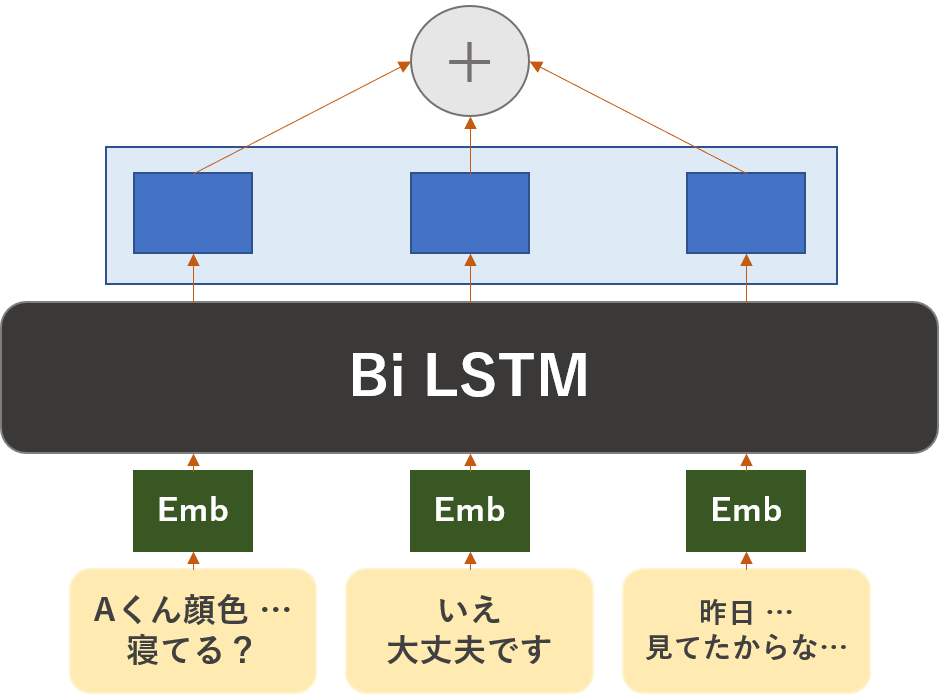
\includegraphics[width=7.0cm]{fig.png}
    \caption{Self-Attention} %タイトルをつける
    \label{fig:sa} %ラベルをつけ図の参照を可能にする
  \end{center}
\end{figure}

ひとまずは情報工学実験 II での実験設定とおおよそ同じで, 図\ref{fig:sa}のように同一 4 コマに含まれているセリフを, 1 文ずつ
Bidirectional LSTM に入力し, 各隠れ層での出力を Self-Attention 層で受け取り, Attention を計算し, タスクとしても同様に感情の 2 値分類 (喜楽 or その他) を解くことを目標とする. 学習パラメータは図\ref{tab:s-A}, ネットワークパラメータは図\ref{tab:net}である. クラス重みは設定していない. 時系列長を 2 - 6 として実験を行った.

\begin{table}[htb]
\begin{center}
\caption{learning parameters}
\begin{tabular}{|c|c|}
\hline
parameter & value \\ \hline
epoch & 100   \\
batch size    & 16    \\
loss & CrossEntropyLoss     \\
optimizer  & Adam     \\
learning rate     & 0.00001  \\ \hline
\end{tabular}
\label{tab:s-A}
\end{center}
\end{table}

\begin{table}[tbh]
\begin{center}
\caption{network parameters}
\begin{tabular}{|c|c|}
\hline
parameter & value \\ \hline
lstm\_in & 300   \\
lstm\_hidden    & 128    \\
self\_atten\_in & $128 \times 2$     \\
atten\_num\_layers & 3     \\ \hline
\end{tabular}
\label{tab:net}
\end{center}
\end{table}

\section{結果}
学習時間については 1 つの時系列長, タッチにつき平均 7 分 / 100 epoch だった.

実験結果を表\ref{tab:result}にまとめた. そして, 情報工学実験 II での LSTM + 3 層 MLP を用いた実験結果との比較を示したのが図\ref{tab:compare}である.

\begin{table*}[!b]
\begin{center}
\caption{result}
\scalebox{0.7}{
\begin{tabular}{cccccccccccccccc|ccc}
\hline
\multirow{2}{*}{seq\_len} & \multicolumn{3}{c}{ギャグ} & \multicolumn{3}{c}{少女漫画} & \multicolumn{3}{c}{少年漫画} & \multicolumn{3}{c}{青年漫画} & \multicolumn{3}{c|}{萌え系} & \multicolumn{3}{c}{5タッチ平均} \\
 & Acc & Recall & F1 & Acc & Recall & F1 & Acc & Recall & F1 & Acc & Recall & F1 & Acc & Recall & F1 & Acc & Recall & F1 \\ \hline
2 & 0.58 & 0.30 & {\ul 0.45} & 0.72 & 0.82 & {\ul 0.70} & 0.53 & 0.42 & 0.45 & 0.71 & 0.21 & 0.53 & 0.58 & 0.36 & 0.53 & 0.62 & 0.42 & {\ul 0.53} \\
3 & 0.36 & 0.50 & 0.33 & 0.70 & 0.87 & 0.68 & 0.48 & 0.42 & 0.42 & 0.69 & 0.43 & 0.59 & 0.56 & 0.41 & 0.52 & 0.56 & 0.52 & 0.51 \\
4 & 0.39 & 0.50 & 0.36 & 0.66 & 0.58 & 0.66 & 0.53 & 0.58 & {\ul 0.48} & 0.69 & 0.36 & 0.57 & 0.63 & 0.50 & {\ul 0.59} & 0.58 & 0.50 & {\ul 0.53} \\
5 & 0.42 & 0.60 & 0.39 & 0.64 & 0.61 & 0.64 & 0.44 & 0.67 & 0.42 & 0.74 & 0.57 & {\ul 0.65} & 0.53 & 0.41 & 0.50 & 0.55 & 0.57 & 0.52 \\
6 & 0.39 & 0.70 & 0.37 & 0.61 & 0.45 & 0.61 & 0.52 & 0.67 & {\ul 0.48} & 0.66 & 0.36 & 0.54 & 0.56 & 0.41 & 0.52 & 0.55 & 0.52 & 0.51 \\ \hline
\multicolumn{1}{l}{ベースライン} & \multicolumn{1}{l}{0.85} & 0 & 0 & 0.43 & 0 & 0 & 0.81 & 0 & 0 & 0.78 & 0 & 0 & 0.66 & 0 & 0 & 0.71 & 0 & 0
\end{tabular}
\label{tab:result}
}
\end{center}
\end{table*}


\begin{figure}[htb]
  \begin{center} %センタリングする
    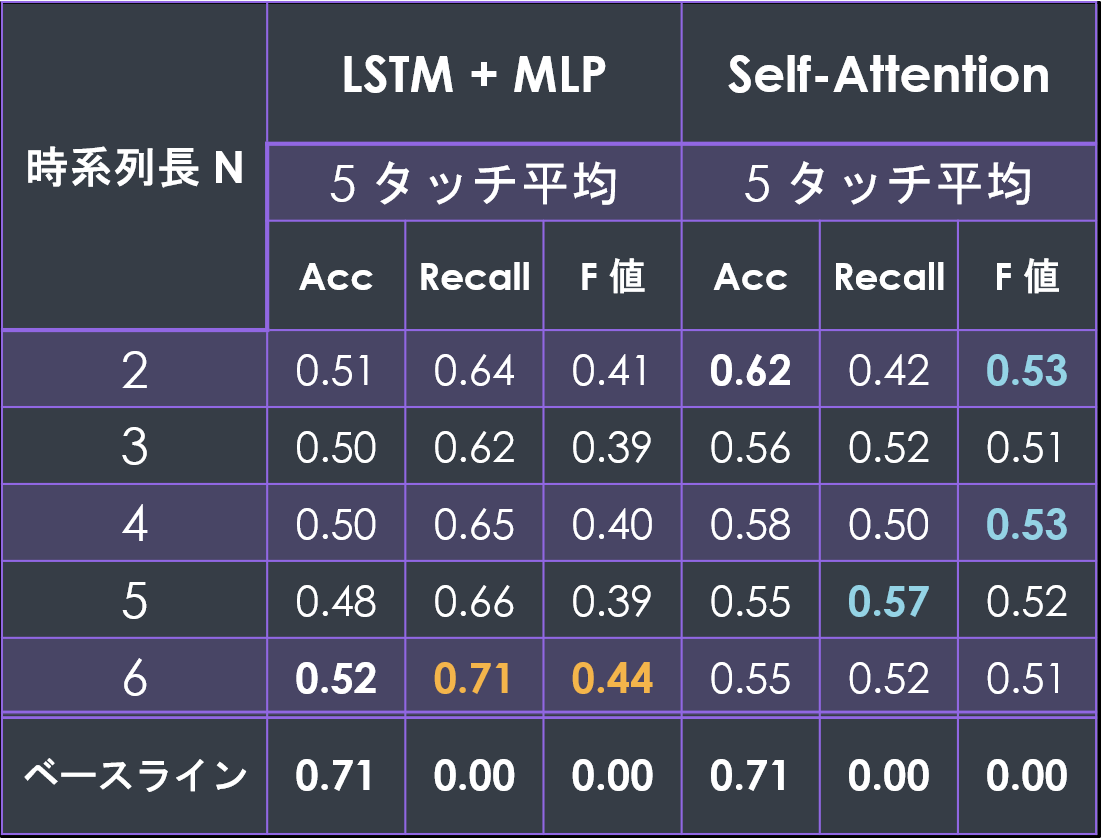
\includegraphics[width=7.0cm]{fig2.png}
    \caption{compare LSTM and Self-Attention} %タイトルをつける
    \label{tab:compare} %ラベルをつけ図の参照を可能にする
  \end{center}
\end{figure}

\section{考察}

どの場合も約 20 epoch 目付近から学習が進んでいない. (result ディレクトリ参照)

LSTM + MLP と比べて, 正例 (喜楽ラベル) の recall は落ち込んだが, Accuracy, F1 値ともに向上した. しかし, 各タッチ ・ 時系列長ごとに見ると, 性能の増減の傾向に差がありその原因については今後詳しく考えていく必要がある.


\section{その他 問題点}
\begin{itemize}
  \item train データを train と validation に分ける際, test は 各タッチの 5 - 10 話を用い, train と validation は 1 - 5 話からランダムに分けているが, データセットの仕様上, 中身が似たようなものになる可能性が高く, 汎化性能に欠ける.
  \item Data Augmentation の手法で日本語 WordNet を用いることで発生する, 意味の乖離.
  \item optuna を用いたハイパーパラメータのチューニングをしていない.
\end{itemize}

\section{課題}
\begin{itemize}
  \item Attention の可視化.
  \item 森先生と大工大の上野先生に 30 話まであるらしい追加データをお願いして, train と validation を話区切りで分けたい.
  \item Data Augmentation の手法の改善案.
  \item optuna でチューニングできるようにする.
  \item BERT の論文等で構造の理解.
  \item 1 文を単語ごとに入力する推定方法も試す.
  \item 現状タッチごとに異なるモデルを作っているので, タッチ情報を表す one-hot-vector 等を用いて 1 つのモデルで性能を確かめることも考える.
\end{itemize}

\section{質問}
Attention 層を複数にする意味
\section{次に読むべき論文}
\begin{itemize}
  \item BERT について書かれているもの.
  \item pointer-generator network について書かれているもの.
\end{itemize}


\bibliographystyle{unsrt}
\bibliography{sankou}
\end{document}
